\chapter{FPGA tervezés}

mi sikerült a hardverből

mentalitás hogy helyes és jól működő chipeket készítsek, inkább a minőségi helyesen működő chip

Rendszer bemutatás top down

\section{Rendszer blokkvázlat bemutatása}

\begin{figure}[H]
	\centering
	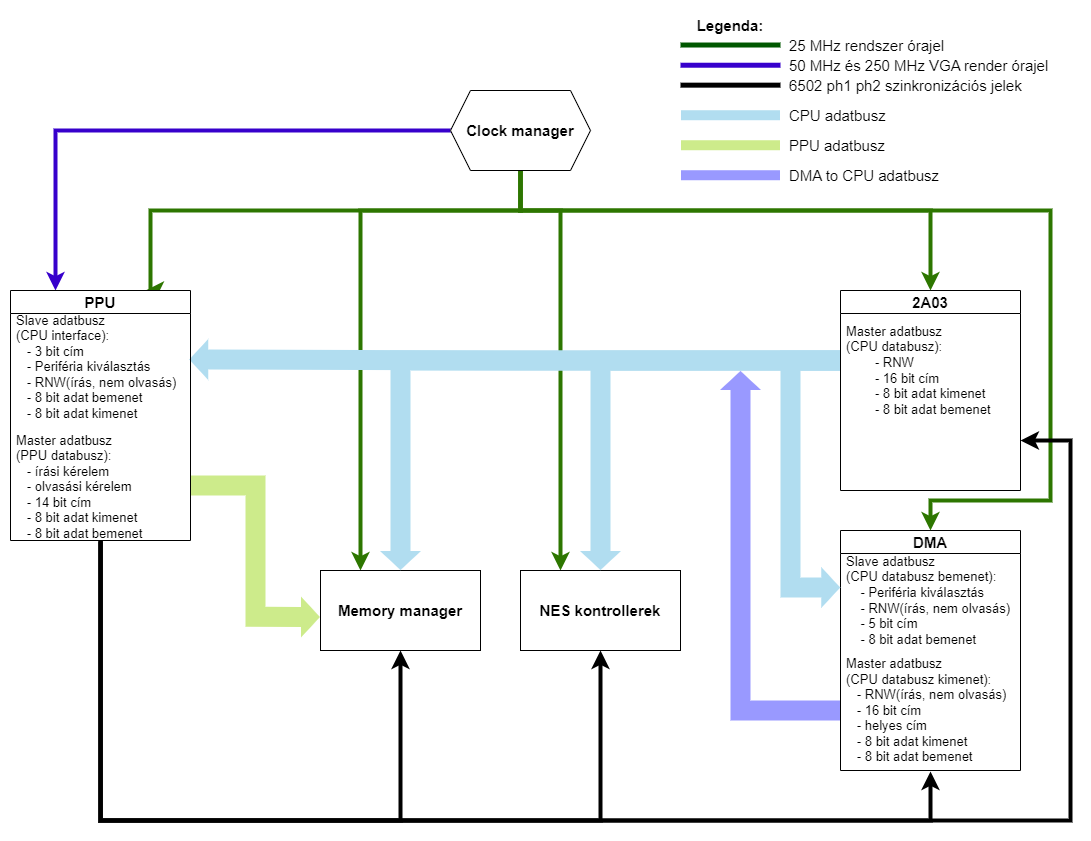
\includegraphics[width=150mm, keepaspectratio]{figures/FPGA-toplevel-diagram}
	\caption{Megvalósult NES top rendszer diagramja} 
	\label{fig:FPGA-toplevel-diagram}
\end{figure}

\section{Működési órajel választása}

\begin{lstlisting}[style=prettyverilog]
reg  clkgen_cnt_en_clr;
wire clkgen_cnt_en_set = (x_rendercntr == (ODDFRAME_END_OF_BG_RENDERING_LINE + 4));

always @(*) 
begin
	if (background_enabled && oddframe && (y_renderingcntr == PRERENDERING_ROW))
		clkgen_cnt_en_clr <= (x_rendercntr == ODDFRAME_END_OF_BG_RENDERING_LINE);
	else
		clkgen_cnt_en_clr <= 1'b0;	
end

// clock genereation enable
reg		clkgen_cnt_en;

always @ (posedge clk)
begin
	if (rst || (x_rendercntr == END_OF_BG_RENDERING_LINE) || clkgen_cnt_en_clr)
		clkgen_cnt_en <= 1'b0;
	else
		if ((x_rendercntr == FIRST_SCANLINE_PIXEL) || clkgen_cnt_en_set)
			clkgen_cnt_en <= 1'b1;
end	

//clock generation timer
reg	[3:0]	clkgen_cnt;

always @ (posedge clk)
begin
	if (rst)
		clkgen_cnt <= 4'd0;
	else
		if (clkgen_cnt_en)
			if (clkgen_cnt == 4'd11)
				clkgen_cnt <= 4'd0;
			else
				clkgen_cnt <= clkgen_cnt + 4'd1;
end

always @ (posedge clk)
begin
	ph1_rising	<= clkgen_cnt_en & (clkgen_cnt == 4'd0);
	ph1_falling <= clkgen_cnt_en & (clkgen_cnt == 4'd5);
	ph2_rising	<= clkgen_cnt_en & (clkgen_cnt == 4'd6);
	ph2_falling <= clkgen_cnt_en & (clkgen_cnt == 4'd11);
end\end{lstlisting}

\section{Picture Process Unit}
\label{sec:PPU-FPGA}

	\subsection{Eredeti rendrelés menete}
	
	\begin{lstlisting}[style=prettyverilog]
	reg [7:0] bg_lsb_buff_reg;
	
	always @ (posedge clk) 
	begin
		if (rst)
			bg_lsb_buff_reg <= 8'd0;
		else
			if (bg_msb_read)
				bg_lsb_buff_reg <= bg_lsb_reg; // shift reg
			else if ((x_rendercntr[1:0] == 2'b11) && (x_rendercntr > START_OF_SHIFT) && (x_rendercntr <= END_OF_SHIFT) && ~(bgrender_state == VBLANK))
				bg_lsb_buff_reg <= {bg_lsb_buff_reg[6:0], 1'b0}; 
	end
	
	reg [7:0] shr_lsb_render = 8'd0;
	wire	  bg_lsb_out;  
	
	always @(posedge clk) 
		if ((x_rendercntr[1:0] == 2'b11) && (x_rendercntr > START_OF_SHIFT) && (x_rendercntr <= END_OF_SHIFT) && ~(bgrender_state == VBLANK))
			shr_lsb_render <= {shr_lsb_render[6:0], bg_lsb_buff_reg[7]};
	
	assign bg_lsb_out = shr_lsb_render[~fh_reg];
	
	reg [7:0] shr_msb_render = 8'd0;
	wire	  bg_msb_out;  
	
	always @(posedge clk) 
		if ((x_rendercntr[1:0] == 2'b11) && (x_rendercntr > START_OF_SHIFT) && (x_rendercntr <= END_OF_SHIFT) && ~(bgrender_state == VBLANK))
			shr_msb_render <= {shr_msb_render[6:0], bg_msb_reg[7]};
	
	assign bg_msb_out = shr_msb_render[~fh_reg];\end{lstlisting}

	\begin{lstlisting}[style=prettyverilog]
	localparam H_SPRITE0_CHECK_END = 4*287 - 1;
	
	reg sprite0_check_reg;
	
	always @(posedge clk)
	begin
		if (rst || (x_rendercntr == H_SPRITE0_CHECK_END))
			sprite0_check_reg <= 0;
		else
			if (x_rendercntr == FIRST_SCANLINE_PIXEL)
				sprite0_check_reg <= 1;
	end
	
	wire sprite0_check = sprite0_check_reg & next_pixel;
	
	wire visible_bg_pixel = |bg_pixel[1:0];
	
	reg [1:0] tile_attr_reg_saved;
	
	always @(posedge clk) 
	begin
		if (rst)
			tile_attr_reg_saved <= 2'b0;
		else
			if (bg_msb_read)
				tile_attr_reg_saved <= tile_attr_reg;
	end
	
	reg [7:0] shr_attr0_render = 8'd0; 
	
	always @(posedge clk) 
		if ((x_rendercntr[1:0] == 2'b11) && (x_rendercntr > START_OF_SHIFT) && (x_rendercntr <= END_OF_SHIFT) && ~(bgrender_state == VBLANK))
			shr_attr0_render <= {shr_attr0_render[6:0], tile_attr_reg_saved[0]};
	
	wire shr_attr0_out = shr_attr0_render[~fh_reg];
	
	reg [7:0] shr_attr1_render = 8'd0; 
	
	always @(posedge clk) 
		if ((x_rendercntr[1:0] == 2'b11) && (x_rendercntr > START_OF_SHIFT) && (x_rendercntr <= END_OF_SHIFT) && ~(bgrender_state == VBLANK))
			shr_attr1_render <= {shr_attr1_render[6:0], tile_attr_reg_saved[1]};
	
	wire shr_attr1_out = shr_attr1_render[~fh_reg];
	
	reg [3:0] bg_pixel;
	
	always @(posedge clk) 
	begin
		if (rst)
			bg_pixel <= 4'b0;
		else
			bg_pixel <= {shr_attr1_out, shr_attr0_out, bg_msb_out, bg_lsb_out};		
	end
	
	wire [4:0] palette_addr = 	(sprite_priority & visible_bg_pixel) ? ({1'b0, bg_pixel}) : ({1'b1, sprite_pixel});
		
	wire tarnsparent_bground = ({bg_msb_out, bg_lsb_out} == 2'b00);
	wire tarnsparent_sprite = (sprite_pixel == 2'b00);
	
	wire sprite_select = (~sprite_priority | tarnsparent_bground) & ~tarnsparent_sprite;

	assign sprite0_hit_set = visible_bg_pixel & sprite0_visible & sprite0_check;\end{lstlisting}

	\subsection{VGA rendelés}

	\subsection{Háttér renderelési állapot gép}

	\subsection{Sprite rendering állapot gép}

	\subsection{CPU által elérhető regiszterek és CPU adatbusz}
	
	\begin{lstlisting}[style=prettyverilog]
	//register write enable signals
	wire control_wr     = ph2_falling & slv_mem_cs & ~slv_mem_rnw & (slv_mem_addr == 3'b000); //CTRL register write #2000
	wire render_mask_wr = ph2_falling & slv_mem_cs & ~slv_mem_rnw & (slv_mem_addr == 3'b001); //MASK register write #2001
	wire oam_addr_wr    = ph2_falling & slv_mem_cs & ~slv_mem_rnw & (slv_mem_addr == 3'b011); //OAM read/write address #2003
	wire oam_data_wr    = ph2_falling & slv_mem_cs & ~slv_mem_rnw & (slv_mem_addr == 3'b100); //OAM data read/write #2004
	wire scrolling_wr   = ph2_falling & slv_mem_cs & ~slv_mem_rnw & (slv_mem_addr == 3'b101); //fine scroll position (two writes: X scroll, Y scroll) #2005
	wire vram_addr_wr   = ph2_falling & slv_mem_cs & ~slv_mem_rnw & (slv_mem_addr == 3'b110); //PPU read/write address (two writes: most significant byte, least significant byte) #2006
	wire vram_data_wr   = ph2_falling & slv_mem_cs & ~slv_mem_rnw & (slv_mem_addr == 3'b111); //PPU data read/write #2007
	
	//Register read enable signals
	wire status_rd      = slv_mem_cs & slv_mem_rnw & (slv_mem_addr == 3'b010);
	wire oam_data_rd    = slv_mem_cs & slv_mem_rnw & (slv_mem_addr == 3'b100);
	wire vram_data_rd   = slv_mem_cs & slv_mem_rnw & (slv_mem_addr == 3'b111);\end{lstlisting}
	
	\subsection{PPU adatbusz és memória elérése}

\section{NES memória felépítése FPGA-ban}

\section{DMA}

\section{6502 processzor működése}

\section{NES kontrollerek kezelése}